\documentclass[output=paper]{LSP/langsci} 
\author{Claudio Fantinuoli}
\abstract{Erfolgreiches Dolmetschen setzt qualifizierte Vorbereitung voraus. Dazu gehören die nutzeradäquate Gestaltung und die kontinuierliche Pflege von Terminologiebe\-ständen sowie die Möglichkeit auf mehrsprachige Informationen und Terminologie schnell und effizient zugreifen zu können. Um die Vorbereitungsphase zu optimieren und zu rationalisieren wird ein dolmetschorientierter Korpus-Ansatz beschrieben und eine dafür entwickelte Terminologie- und Wissensmanagementsoftware vorgestellt. Für die Konferenzvorbereitung implementiert die Software Funktionalitäten wie automatische Termextraktion, automatische Herstellung von Fachkorpora und die Möglichkeit der Informationssuche aus strukturierten Webressourcen. Darüber hinaus bietet das Tool Module zur Verwaltung der gewonnenen Informationen und zum dolmetschfreundlichen Abrufen der in Glossaren fixierten Terminologiebestände.
In diesem Artikel sollen die relevanten Grundlagen der Dolmetschwissenschaft und einige Module der implementierten Software vorgestellt werden.}

\title{Computerlinguistik in der Dolmetschpraxis unter besonderer Berücksichtigung der Korpusanalyse} 
\shorttitlerunninghead{Computerlinguistik in der Dolmetschpraxis}

\maketitle

\begin{document}

\begin{otherlanguage}{ngerman}
%\setcounter{page}{1}



\section{Der Dolmetscher und der Dolmetscherberuf}\label{sec:fantinuoli:1}

Dolmetscher arbeiten per definitionem in einem multilingualen Umfeld. Sie übertragen einen mündlich dargebotenen Text von einer Ausgangsprache in eine Zielsprache und dienen dem unmittelbaren Verständnis der am Kommunikationsprozess beteiligten Teilnehmer.

Grundsätzlich wird zwischen drei Formen des Dolmetschens unterschieden: dem Gesprächsdolmetschen, dem Konsekutivdolmetschen und dem Simultandolmetschen. Beim Gesprächsdolmetschen -- je nach Einsatzbereich, Setting und Land auch „Gerichtsdolmetschen“, „Verhandlungsdolmetschen“, „Community Interpreting“, „Kommunaldolmetschen“ oder „Fachdolmetschen“ genannt -- findet die Übertragung eines Textes bidirektional zwischen mindestens zwei Kommunikationspartnern statt, die in einer dialogischen Interaktion sukzessiv von Textproduzenten zu Textrezipienten werden. Beim Konsekutivdolmetschen findet die Übertragung eines Textes dagegen in einer meist nicht dialogischen Interaktion monodirektional von einer Sprache in die andere statt. Dies geschieht zeitversetzt, und zwar nachdem der Textproduzent den gesamten Text oder einen Teil davon zu Ende vorgetragen hat. Auch beim Simultandolmetschen wird der Text monodirektional in die Zielsprache übertragen, jedoch (fast) gleichzeitig zu seiner Äußerung.\footnote{Die Zeitversetzung zwischen Äußerung und Verdolmetschung wird in der Dolmetschwissenschaft „Decalage“ genannt und beträgt einige Sekunden (vgl. \citealt{Pöchhacker2004}).} Um die Simultanität der Übertragung zu ermöglichen, bedienen sich Dolmetscher technischer Einrichtungen, d.h. schalldichten Kabinen, Kopfhörern und Mikrophonen. Aufgrund des typischen Settings -- Kongresse, Tagungen, Seminare, usw. --, in dem sie Anwendung finden, werden das Konsekutiv- und Simultandolmetschen traditionell auch als Konferenzdolmetschen bezeichnet. 

Die hier aufgeführte Unterscheidung und Bezeichnung der Hauptdolmetschformen sind keineswegs als exhaustiv oder definitiv zu betrachten. Vielmehr bewegt sich jede Form des Dolmetschens in einem begrifflichen Kontinuum zwischen Konferenzdolmetschen (KD) und Nicht-Konferenzdolmetschen (NKD).\footnote{Zur weiteren Differenzierung und Annäherung zwischen den vielen Typologien von Dolmetschformen vgl. \citet[25ff]{Feldweg1996}, \citet[51]{Kalina2001}, \citet[33]{Pöchhacker2000} und \citet[354ff]{Gross-Dinter2009}} In diesem Beitrag wird insbesondere auf das Konferenzdolmetschen eingegangen. Ein besonderes Augenmerk gilt dabei dem Simultandolmetschen, der gegenwärtig am häufigsten eingesetzten Form des Konferenzdolmetschens.

Die Heterogenität und Spezifität der Konferenzthemen verlangt von den Dolmetschern, in der Regel keine Experten des auf der Konferenz behandelten Faches,  die Bereitschaft und Fähigkeit, sich ständig in neue Fachgebiete einzuarbeiten (vgl. \citealt{Kalina2007,Andres2011}). Für die Vorbereitung steht den Dolmetschern meist sehr wenig Zeit zur Verfügung, da innerhalb eines relativ kurzen Zeitraumes mehrere thematisch unterschiedliche Einsätze bewältigt werden müssen. So gehört es beispielsweise zum Alltag der Dolmetscher, dass sie sich innerhalb nur weniger Tage auf eine Bilanzpressekonferenz, eine technische Schulung und ein medizinisches Symposium vorbereiten müssen. Sehr oft findet das erworbene Wissen nur für einen einzelnen Einsatz Verwendung. Auf internationalen Fachkonferenzen wird die Kommunikation unter den Experten, die zwar ein entsprechendes Fachwissen, jedoch keine gemeinsame Sprache miteinander teilen, durch zumeist fachfremde Personen -- die Dolmetscher -- ermöglicht. Aus der Perspektive der stattfindenden Kommunikation entsteht dabei eine Laien-Experten-Konstellation (vgl. \citealt{Will2009}). Generell manifestiert sich das daraus resultierende Ungleichgewicht auf drei Ebenen:

\begin{itemize}
\item 
Inhalt
\item 
Terminologie
\item 
Phraseologie
\end{itemize}

Die inhaltliche Ebene betrifft das Fachwissen. Die Kommunikation unter den Konferenzteilnehmern basiert auf einem hohen Grad an Vorwissen, das in unterschiedlichem Maße von den Textproduzenten und Textrezipienten geteilt wird. Ohne dieses Wissen kann die Kommunikation nicht stattfinden, da Schlüsselkompetenzen fehlen, die erforderlich sind, um Sachverhalte richtig zu verstehen. Die terminologische Ebene betrifft die Fachterminologie, d.h. die Gesamtheit aller Fachtermini, die einem oder mehreren Gebieten zugeordnet werden können und die auf einer Konferenz verwendet werden, um fachliche Informationen auszutauschen. Nur mit der richtigen Terminologie kann eine reibungslose Fachkommunikation stattfinden, da diese in allen Fachbereichen die Grundlage der schriftlichen und mündlichen Fachkommunikation bildet (vgl. \citealt[6]{Arntz2009}). Die phraseologische Ebene betrifft die fachgebundene Ausdrucksweise, die durch die sogenannten „Fachwendungen“ \citep[207]{Picht1990} ihren Ausdruck findet. Unter Fachwendungen versteht man die Verbindung von mindestens zwei sprachlichen Elementen zur Äußerung eines fachlichen Inhaltes. Rossenbeck beschreibt diese Fachwendungen -- auch Fachphraseologie genannt -- als „die Gesamtheit der Wortbildungen, deren Bestandteile sich zu einer charakteristischen Kombination verfestigt haben und die in Texten eines bestimmten Fachgebiets zu beobachten sind“ \citep[199]{Rossenbeck1989}. Bei der phraseologischen Ebene geht es um die Wahl bestimmter Ausdrücke, Phrasen, Kollokationen, etc., die typischerweise von den Konferenzteilnehmern verwendet werden. Da sich auf derartigen Veranstaltungen Insider eines Fachgebietes einfinden, verwenden diese einen bestimmten „in-house jargon“ \citep[777]{Kalina2005}, eine eigene gemeinsame Fachsprache. Beispiele hierfür sind spezifische Verbalverbindungen des Typs \textit{Abtragspartikeln ausschwemmen}, \textit{ein Testament errichten} und \textit{eine Aktie zeichnen}. 

Um der fachlichen Kommunikationssituation gerecht werden zu können, müssen Dolmetscher folglich alle drei Ebenen gut beherrschen. Sie müssen über genügend fachliches Vorwissen verfügen, um die Zusammenhänge (schnell) erfassen und Informationen von einer Sprache in eine andere übertragen zu können. Sie müssen die verwendete Terminologie in den zu verdolmetschenden Sprachen kennen und parat haben, um den reibungslosen und eindeutigen mehrsprachigen Informationsaustausch adäquat zu ermöglichen. Schließlich müssen Dolmetscher auch die phraseologischen Elemente beherrschen, damit sie von den Zuhörern als Insider und letztendlich als fachkundig wahrgenommen werden.

Wenn Dolmetscher nicht selbst Fachleute in einem spezifischen Konferenzthema sind -- was aufgrund der hohen kunden- und themenspezifischen Varianz sehr wahrscheinlich ist -- müssen sie sich die drei aufgeführten Ebenen systematisch erschließen. In Anbetracht der Spontaneität und der zeitlichen Begrenzungen der im Dolmetschprozess stattfindenden Kommunikation ist es im Gegensatz zum Übersetzen notwendig, diesen Erschließungsprozess zu antizipieren, d.h. ihn in die Vorbereitungsphase zu verlagern (vgl. \citealt{Gile1995,Stoll2009,Will2009}).

Um die Dolmetscher bei der Erschließung und Anwendung der drei genannten Wissensebenen zu unterstützen und generell die Rationalisierung des Dolmetschprozesses zu fördern, können Computeranwendungen eingesetzt werden. In den nachfolgenden Abschnitten werden die theoretischen Grundlagen zum Thema Terminologie- und Wissensmanagement im Bereich Dolmetschen kurz skizziert, die heute den Dolmetschern zur Verfügung stehenden Software analysiert und die möglichen Vorteile von korpuslinguistischen Ansätzen bei der Vorbereitung von Fachkonferenzen angesprochen. Im Anschluss daran wird schließlich eine Wissens- und Terminologie-Software namens InterpretBank vorgestellt, die speziell für Dolmetscher entwickelt wurde.

\section{Wissen und Terminologie für Dolmetscher}\label{sec:fantinuoli:2}

Das Thema Wissens- und Terminologiemanagement sowie Einsatz von Computeranwendungen beim Dolmetschen hat erst in den letzten Jahren -- wenn auch in geringem Maße -- Eingang in die dolmetschwissenschaftliche Literatur gefunden. Um einen Überblick zu geben, werden in diesem Kapitel die wichtigsten Arbeiten zu diesen Themen chronologisch vorgestellt.

\citet{Fantinuoli2006} fokussiert das terminologische Problem beim Dolmetschen auf die Notwendigkeit, qualitativ hochwertige sprachliche und nicht-sprachliche Ressourcen \textit{ad-hoc} zu erstellen, da Dolmetscher aufgrund der Variabilität und Spezifität der von ihnen zu behandelnden Themen über keine vorgefertigten Ressourcen verfügen können. Dabei greift er auf computerlinguistische Anwendungen zurück und stellt den Ansatz der \textit{Corpus Driven Interpreter Preparation} als Methode vor, um die in \sectref{sec:fantinuoli:1} genannten und für den Erfolg eines Dolmetscheinsatzes notwendigen Wissensebenen zu erschließen. Dieser Ansatz basiert auf dem Gebrauch korpuslinguistischer Anwendungen, in erster Linie Software zur einsprachigen Konkordanzanalyse, die den Vorbereitungsprozess unterstützen sollen:

\begin{quote}
To facilitate this process, we propose an approach to “Corpus Driven Interpreters Preparation”. The process of “knowledge/language learning” needed by interpreters in order to prepare themselves for a conference can be optimized if “terminology driven”, i.e., “bottom-up”: from the terminology to the conceptual structure of a particular domain \citep[174]{Fantinuoli2006}.
\end{quote}

Da bei Konkordanzprogrammen ein Wort oder eine Phrase zur nächsten führen kann -- abhängig von Intuition, Kompetenz, Interessen und Bedürfnissen eines Nutzers -- können Korpora als Quelle eines unendlichen serendipity process \citep{Johns1988} betrachtet werden. Ausgehend von einer kleinen Anzahl an themenspezifischen Termini können Dolmetscher ein einsprachiges, themenspezifisches Fachkorpus „erforschen“ und dabei lernen, wie sich ein Terminus innerhalb einer Domäne verhält, welche Bedeutungen er haben kann, etc. All dies geschieht mit einer „flexibility and active interaction typical of the interpreter's preparation“  \citep[174]{Fantinuoli2006}.

\citet{Rütten2007} beschreibt den Terminologiebedarf der Dolmetscher als Teil des Informations- und Wissensmanagements im Bereich Konferenzdolmetschen und verfolgt das Ziel, die Rolle von Information und Wissen sowie entsprechende Zusammenhänge deutlich zu machen. Nachdem sie die wichtigsten Theorien dieser zwei Teildisziplinen näher beschreibt, schlägt sie eine Brücke zu den gängigen Dolmetschtheorien im Bereich Wissenskonstituierung wie z.B. zu den \textit{Phasen} von \citet[778]{Kalina2005} und plädiert für die Darstellung dieses Wissens nach Wüster \citep[83]{Rütten2007} anhand von Benennung, Begriff und Begriffsbeziehung. Die von ihr vorgeschlagene Darstellung von Zusammenhängen zwischen Dolmetschprozess und Wissen erläutert sie anhand einer Fallstudie, in der sie die Vorbereitungsarbeiten im Hinblick auf den informations- und wissensbezogenen Arbeitsablauf analysiert. Auf der Basis dieser Erkenntnisse schildert sie schließlich die Struktur eines Softwaremodells zur Unterstützung des Arbeitsablaufs.

\citet{Stoll2009} beschreibt ein Modell der Vorverlagerung von Kognition aus der Phase des Simultandolmetschens in die Phase der Vorbereitung. Dabei tritt er für eine intensivere Auseinandersetzung mit dem Thema der Vorverlagerung des Denkaufwandes aus der Simultanphase ein, da sie zu einer Qualitätssteigerung führen kann. Er stützt sich dabei auf die in der Dolmetschwissenschaft anerkannte These, dass die fachliche Vorbereitung im Vorfeld stattfinden müsse und Dolmetscher in dieser Phase so viel Wissen wie möglich erwerben müssten \citep[147]{Gile1995}, denn dies sei schließlich während der Konferenz nicht möglich. Dank der Vorverlagerung des kognitiven Aufwandes könnten Konzentrationsressourcen währen der Verdolmetschung freigesetzt werden, die dann z.B. auch für die Bedienung einer terminologischen Software während des Simultandolmetschens zur Verfügung stünden \citep[49]{Stoll2002}.

\largerpage
\citet{Will2009} setzt sich mit Modellen und Methoden auseinander, die notwendig sind, um die strukturellen Prozesse der Organisation terminologischer Arbeit für Dolmetscher zu definieren. Er beschreibt die komplexen Wissenskonstellationen, die für den Erfolg einer Dolmetschleistung grundlegend sind und entwickelt die in fünf Etappen zusammengefasste dolmetschorientierte Terminologiearbeit (DOT). Will bedient sich dabei des kontextspezifischen Terminus-Modells nach \citet{gerzymisch1996termini}, das im Gegensatz zu Wüsters kontextunabhängiger, eindeutiger Zuordnung von Begriff und Bedeutung (Systemebene) auch die Möglichkeit von Abweichungen (Individualebene) vorsieht. Ausgehend von der Kritik an der Praxis, vor einem Dolmetscheinsatz einfache zusammenhanglose Wortlisten zu erstellen, die oft zu Fehlentscheidungen führen können, etwa wenn Polyseme oder Terminologisierungen auftreten \citep[6]{Will2009}, plädiert Will für eine „Detektivarbeit“, die -- anders als bei punktuellen Glossaren -- Wissen im Zusammenhang, d.h. im Kontext, abbildet. Bei dieser Detektivarbeit wird zunächst ein Wort (Benennung) als Begriff (Definition) erschlossen, um zu erkennen, welchem Wissensbereich der Terminus zugeordnet werden kann (vgl. \citealt{Will2010}). Nur so könne eine sichere und adäquate Verdolmetschung ermöglicht werden.

In seiner Arbeit über terminologische Probleme beim Medizindolmetschen konstatiert Gorjanic schließlich, wie „Communication problems often arise from insufficient knowledge of terminology rather than a lack of general language skills“ \citep[85]{Gorjanc2009}. Er geht von \citet{Fantinuoli2006} These zur Ressourcenknappheit aus und behauptet, dass Dolmetscher Strategien entwickeln müssen, um Datenbestände für das jeweilige Thema selbst zu erarbeiten. Dies kann durch spezialisierte Anwendungen zur Vorbereitung und Analyse sprachlicher Ressourcen sowie zur Speicherung und Verwaltung der Ergebnisse eines solchen Verfahrens erzielt werden. Aus dieser Notwendigkeit heraus kommt er zu dem Schluss, „the educational process includes information on terminology management options based on text resources” \citep[89]{Gorjanc2009}.

\section{Nutzungsverbreitung von Computeranwendungen unter den Dolmetschern}\label{sec:fantinuoli:3}

Seit den 90er Jahren wurden unter Konferenzdolmetschern zahlreiche Umfragen zu deren Erfahrung mit dem Computereinsatz in ihrem dolmetschbezogenen Berufsleben durchgeführt. All diese Umfragen hatten zum Ziel, die Verbreitung von Programmen zur Terminologieverwaltung zu analysieren. Die in den letzten Jahren durchgeführten Umfragen (vgl. \citealt{Valentini2002,Honegger2006,SDI2007,Bilgen2009}) zeigen hinsichtlich der Verbreitung der für Dolmetscher entwickelten Werkzeuge ein ernüchterndes Bild. Für die Terminologieverwaltung verwenden die meisten Befragten -- wenn überhaupt -- immer noch traditionelle Lösungen wie z.B. Textverarbeitungs- und Tabellenkalkulationsprogramme (z.B.\textit{ MS-Word} oder \textit{MS-Excel}); nur selten werden Programme verwendet, die auch eine Simultanmodalität besitzen. Keiner der Befragten erwähnt korpuslinguistische Anwendungen, wie beispielsweise Konkordanz-Software, Tools zur Korpuserstellung, Terminologieextraktion, Wissenserschließung, etc. Dennoch zeichnet sich seit einigen Jahren ein stetig wachsendes Interesse für Methoden und praktische Anwendungen ab, die die Vorbereitung, Durchführung und Nachbearbeitung eines Dolmetscheinsatzes effizienter gestalten sollten. Das wachsende Interesse spiegelt sich auch in der Zahl dolmetschwissenschaftlicher Publikationen wider (siehe \sectref{sec:fantinuoli:2}), die zu diesem Thema veröffentlicht wurden.

\section{Ressourcen und Tools für Dolmetscher}\label{sec:fantinuoli:4}
\largerpage

Es ist allgemein bekannt, dass das Internet die vertrauteste und nutzerfreundlichste Arbeitsumgebung für Übersetzer und Dolmetscher ist \citep{Zanettin2002}. Man kann zu Recht davon ausgehen, dass alle Dolmetscher und Übersetzer heutzutage das Medium Internet als wichtigste Quelle für die Beschaffung von Informationen und Terminologie zu einem bestimmten Thema nutzen. Internetsuchmaschinen bieten in erster Linie die Möglichkeit, eine fast unendliche Menge an ein- oder mehrsprachigen Texten über alle erdenklichen Fachgebiete zu finden, die -- zusammen mit den konferenzspezifischen Texten, die vom Konferenzorganisator oder \textit{Chef d'équipe} zur Verfügung gestellt werden -- als Grundlage für die Vorbereitung einer Konferenz dienen. Dabei geht es um Paralleltexte, d.h. thematisch verwandte Texte in der Zielsprache, die zur Erschließung linguistischer und nicht-linguistischer Elemente verwendet werden können, wie z.B. die Suche nach Äquivalenten eines Terminus in einer anderen Sprache. Das Internet bietet darüber hinaus zahlreiche, oft kostenlose Möglichkeiten, strukturierte Informationen zu einem bestimmten Thema zu finden. Dies ist beispielsweise bei allgemeinen Enzyklopädien wie Wikipedia\footnote{\url{http://www.wikipedia.org}} der Fall, wo Einträge zu einer nahezu unbegrenzten Anzahl von Themen enthalten sind, oder bei fachspezifischen Ressourcen wie z.B. der Wissensdatenbank Phenowiki\footnote{\url{http://www.phenowiki.org}}, die Informationen über psychiatrische Erscheinungen zum Inhalt hat. Auch die Anzahl der terminologischen und lexikografischen Ressourcen -- sowohl ein- als auch mehrsprachige -- ist sehr groß. Man denke nur an terminologische Datenbanken wie IATE\footnote{\url{http://www.iate.europa.eu}}, die mehrsprachige Terminologie-Datenbank der EU, kollaborative Internetseiten zur Speicherung von Übersetzungen wie Leo\footnote{\url{http://www.leo.de}}, oder lexikografische Ressourcen wie DWDS\footnote{\url{http://www.dwds.de}}.

Anders als das Internet, das immer mehr Ressourcen bietet, die für Dolmetscher und Übersetzer nützlich sind, ist die Anzahl der dolmetschspezifischen Software -- im Gegensatz zur Übersetzungsbranche, in der sich viele Software zur Unterstützung des Übersetzungsprozesses etabliert haben -- in Zahl, Funktionsumfang und Verbreitung sehr begrenzt. Die Gründe hierfür sind vielfältig. Einerseits ist der Konferenzmarkt im Vergleich zum Übersetzungsmarkt wesentlich kleiner (kleinere Anzahl der praktizierenden Dolmetscher und kleinere Auftragsvolumina), so dass das wirtschaftliche Interesse der Softwarehersteller sehr gering ist. Andererseits fehlt das Bewusstsein seitens der Dolmetscher, dass durch ein besseres Management der zur Verfügung stehenden Ressourcen eine höhere Wettbewerbsfähigkeit und eine bessere Qualität der erbrachten Leistungen erzielt werden können. Dies könnte an den „schwer erfassbaren Arbeitsbedingungen, unter denen Dolmetscher mit Texten konfrontiert werden“ \citep[19]{Will2009} liegen.

 
Die meisten dolmetschspezifischen Software, die im Laufe der Jahre entwickelt wurden, sind rein terminologische Datenbanken: Sie dienen ausschließlich der Speicherung und Verwaltung mehrsprachiger Glossare. Im Gegensatz zu den Terminologiesystemen für Übersetzer zeichnen sie sich meistens durch eine vereinfachte Eintragsstruktur und durch die Implementierung einer Funktionalität zum Abrufen der Glossare in der Kabine aus (ähnlich wie bei den elektronischen Wörterbüchern). Zu den Lösungen, die für Dolmetscher entwickelt wurden, gehören Interplex\footnote{\url{http://www.fourwillows.com/interplex}}, Terminus\footnote{\url{http://www.terminus.wintringham.ch}}, Lookup\footnote{\url{http://www.lookup-web.de/}} und TermDB\footnote{ TermDB wurde von einem AIIC-Konferenzdolmetscher entwickelt und nie kommerziell vertrieben.}. Alle Lösungen ermöglichen das Anlegen und die Verwaltung mehrsprachiger Wortlisten und bieten Felder für das Eintragen von Zusatzinformationen. Außer der Einteilung in Glossaren bieten sie -- mit Ausnahme von Interplex -- einige weitere Kategorisierungsmöglichkeiten wie z.B. Konferenz, Thema oder Kundenzuordnung. Die Suche nach einem Wort erfolgt meist durch Eingabe einer Zeichenkette in das Suchfeld und durch Drücken der Eingabetaste. Keine der oben genannten Software nutzt allerdings computerlinguistische Ansätze, um die Suchfunktion kabinenfreundlicher zu gestalten. So ermöglicht keine dieser Software in der uns vorliegenden Version eine Reduzierung der Trefferquote z.B. durch Stopwords oder durch eine Fehlerkorrektur im Falle eines Tippfehlers/Rechtschreibfehlers im Glossar; beide sind allerdings wichtige Eigenschaften für die \textit{Usability} einer simultanfähigen Software (siehe \sectref{sec:fantinuoli:6.3}).

Einige Sprachendienste internationaler Unternehmen oder Institutionen haben im Laufe der Jahre eigene Lösungen entwickelt. Eine erwähnenswerte Anwendung für Dolmetscher ist Lithos, die terminologische Software der Generaldirektion Dolmetschen der Europäischen Union. Anders als bei den oben genannten Programmen handelt es sich bei Lithos um eine Server-Client-Anwendung zur Verwaltung und Bereitstellung mehrsprachiger Glossare, die von den fest angestellten und freiberuflichen Dolmetschern der EU eingesetzt werden kann. Lithos liegt eine Datenbank zugrunde, die alle 24 EU-Amtssprachen umfasst. Des Weiteren sind Felder zur thematischen Einordnung der Einträge und deren Zuweisung zu einem bestimmten Glossar vorgesehen. Die auf einem zentralen Server gespeicherte Datenbank von Lithos wird monatlich durch Ergänzung der zuletzt vom SCIC-Terminologiedienst veröffentlichten Glossare aktualisiert. Abgesehen vom direkten Online-Zugang über einen Internetbrowser unterstützt Lithos die Installation eines Clients auf dem Rechner des Nutzers zur Anwendung der Datenbank im Offline-Modus. Die Offline-Datenbank kann jederzeit aktualisiert und somit auf den Stand der Online-Version gebracht werden.

\section{Computer- und Korpuslinguistik in der Dolmetschpraxis}\label{sec:fantinuoli:5}

Im Gegensatz zu allgemeinen und dolmetschspezifischen Programmen zur Terminologieverwaltung, die unter Dolmetschern heutzutage einen gewissen Bekanntheitsgrad erreicht haben, haben korpuslinguistische Ansätze bis heute so gut wie keine Resonanz im Bereich des Dolmetschens gefunden. Einzige Ausnahme stellt die deskriptive Dolmetschwissenschaft dar, die seit einigen Jahren mit den so genannten \textit{Corpus-Based Interpreting Studies} nach Erkenntnissen über unterschiedlichste Aspekte des Dolmetschens sucht. Einige Beispiele dafür sind Studien zur Direktionalität beim Simultandolmetschen \citep{Bendazzoli2005}, zu Strategien beim Simultan- und Konsekutivdolmetschen in Bezug auf Eigennamen \citep{Meyer2008}, oder zu den Implikationen des Einsatzes nicht professioneller Dolmetscher im Gesundheitswesen \citep{MeyerEtAl2010}. Die Gründe für die zeitliche Verzögerung des Einzugs der Korpuslinguistik in die Dolmetschpraxis und in die Dolmetscherausbildung sind vielfältig. Mit wenigen Ausnahmen 
\citep{Fantinuoli2006,Gorjanc2009} hat sich die Dolmetschwissenschaft einerseits noch nicht mit den Möglichkeiten auseinandergesetzt, die die Computer- und Korpuslinguistik für die Praxis des Dolmetschens und für die Ausbildung angehender Dolmetscher bietet; andererseits fehlen spezifische computerlinguistische Anwendungen, die genau auf die Bedürfnisse der Dolmetscher zugeschnitten sind. Die Computer- und Korpuslinguistik kann für die Dolmetschpraxis und -ausbildung jedoch einen wichtigen Beitrag leisten. Bei angehenden Dolmetschern können Lernerkorpora, zum Beispiel aus politischen Reden, Antworten zu den sprachlichen Besonderheiten dieser Sprache liefern, vor allem in Bezug auf die Verdolmetschung in die Fremdsprache. Der Lerner wird somit emanzipiert und die Lernautonomie gefördert. Bei professionellen Dolmetschern kann sie insbesondere für eine Optimierung der Vorbereitungsphase sorgen, indem sie gezielte Informationen und Darstellungsformen zu einem bestimmten Fachthema bereitstellt. Die gewonnenen sprachlichen und nicht-sprachlichen Daten können systematisiert und für zukünftige Projekte wiederverwendet werden, was die Wirtschaftlichkeit der einzelnen Dolmetscheinsätze langfristig erhöht (siehe \sectref{sec:fantinuoli:6}). 

Um die Bedeutung eines Fachterminus besser zu verstehen und diesen korrekt und nutzeradäquat zu verwenden, ist es zum Beispiel möglich, aus einem themenspezifischen einsprachigen Fachkorpus reelle Verwendungsbeispiele zu visualisieren. Die Einbeziehung der aktuellen Realisierung von Termini und Phrasen in Originaltexten ist die Voraussetzung dafür, dass „Termini im Kontext beschrieben und mit ihrer Systembedeutung verglichen werden können“ \citep[42]{Will2009}. Das Nachschlagen in Parallelkorpora kann darüber hinaus eine unerschöpfliche Quelle an Übersetzungsvorschlägen sein. Für diese Art der Informationsgewinnung aus Korpora eignet sich die klassische Form der Darstellung von korpuslinguistischen Befunden, das so genannte \textit{Key Words in Context}. Die geordnete Darstellung von Konkordanzen ermöglicht es dem Nutzer, zu neuen Erkenntnissen über Sprache und Inhalt zu gelangen. Der Prozess der Korpusanalyse kann außerdem dazu beitragen, vorhandene Kenntnisse zu verfestigen \citep{Johns1991} und erscheint somit geeignet, Dolmetscher vor einem Dolmetscheinsatz bei der Aktivierung ihres Vorwissens zu unterstützen (siehe \sectref{sec:fantinuoli:2}). Die Wichtigkeit dieser „contextual patterns“ \citep[15]{Aston2001} im Bereich der aktiven Sprachbeherrschung wird in vielen wissenschaftlichen Arbeiten thematisiert.\footnote{Eine ausführliche Einführung bietet hierzu \citet{Aston2001}.} Hier ist auch die Kernidee der \textit{Corpus Driven Interpreter Preparation} \citep{Fantinuoli2006} angesiedelt. Ergänzt durch weitere Informationen inhaltlicher und sprachlicher Natur (siehe \sectref{sec:fantinuoli:6.1.4}), die auf einer zentralen Benutzeroberfläche dargestellt werden, kann die Analyse eines Fachkorpus dazu beitragen, die drei in \sectref{sec:fantinuoli:2} definierten Wissensebenen zu erlangen. Dies wird ermöglicht, indem das Korpus und die Konkordanzen als Quellen für einen unendlichen \textit{serendipity process} \citep{Johns1988} benutzt werden, da ein Wort zum nächsten führt, abhängig von Intuition, Kenntnissen, Interessen und Bedarf des Nutzers \citep{Bernardini2001}. Dieser Ansatz findet offensichtlich auch bei Will Zuspruch, denn er konstatiert:

\begin{quote}
Diese Detektivarbeit ist deswegen von Bedeutung, weil sie [\ldots] Wissen im Zusammenhang abbildet, wobei dieser Zusammenhang auf weitere Termini, auch aus verschiedenen Texten, ausgeweitet werden kann und sollte \citep[53]{Will2010}.
\end{quote}

Ähnlich wie beim Spracherwerb steht die Verwendung von Korpora in der Dolmetschvorbereitungsphase im Einklang mit dem klassischen affektiven Prinzip des emotionalen und nicht nur rationalen Lernansatzes, der in den letzten Jahren im Mittelpunkt des wissenschaftlichen Diskurses im Bereich des fremdsprachlichen Spracherwerbs stand \citep[240]{balboni_sfide_2002}.


\begin{figure}
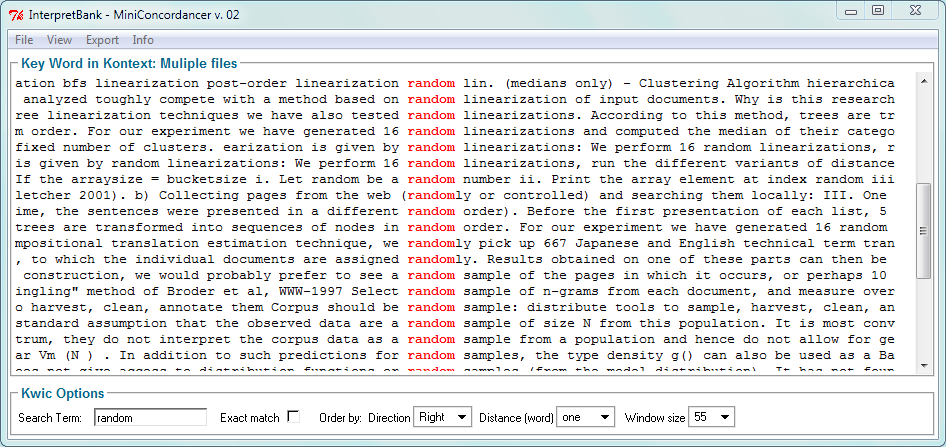
\includegraphics[width=\textwidth]{figures/FantinuoliF1.png}
\caption{Einsprachige Konkordanzen}
\label{fig:fantinuoli:1}
\end{figure} 

Im Bereich Spracherwerb und Übersetzungsdidaktik ist die Hauptidee, den Lernenden in ein aktives Mitglied des  Lernprozesses zu verwandeln \citep{Kiraly2000} und den Lernprozess datenbasiert anstatt regelbasiert zu gestalten. In diesem Zusammenhang beschreibt \citeauthor{boultondatadriven2009} das Data Driven Learning (DDL) mit folgenden Worten:


\begin{quote}
DDL typically involves exposing learners to large quantities of authentic data -- the electronic corpus -- so that they can play an active role in exploring the language and detecting patterns in it. They are at the centre of the process, taking increased responsibility for their own learning rather than being taught rules in a more passive mode (\citeyear[82]{boultondatadriven2009}). 
\end{quote}

DDL steht wiederum im Einklang mit dem Spracherwerbsansatz von \citet{odlin_printout_1994}. 
Seiner These nach können die Merkmale einer Sprache mittels eines Konkordanzprogramms und der daraus resultierenden Arbeit mit echten Verwendungsbeispielen erlernt werden. Das Experimentieren mit Korpora bietet “virtually unlimited opportunities for learning by discovery, as learners embark on challenging journeys whose outcomes are unpredictable and usually rewarding” \citep[246]{Bernardini2001}. Der Lerner wird somit zur Hauptfigur des Lernprozesses. Bei der Einsatzvorbereitung kann der Dolmetscher ähnlich wie der Sprachlerner eine größere Autonomie bei der Suche und Verifizierung der eigenen Übersetzungsvorschläge erlangen. Korpora können in der Tat eine hilfreiche Quelle für Terminologie und faktische Informationen sein. Dies gilt sowohl für Übersetzer \citep{friedbichler_potential_2000,Zanettin2002,castagnoli_wacky_2006,Hansen-Schirra2008} als auch für Dolmetscher.

Nachdem die ersten theoretischen Arbeiten im Bereich linguistischer und extra-linguistischer Vorbereitungsstrategien professioneller Dolmetscher erschienen sind,\footnote{Hierzu die \textit{Corpus Driven Interpreter Preparation} von \citet{Fantinuoli2006} und die \textit{Dolmetschorientierte Terminologiearbeit} von \citet{Will2009}.} die etwas Licht auf den terminologischen Bedarf der Dolmetscher geworfen haben, wurde der Versuch unternommen, ein korpuslinguistisches Instrumentarium für diese Zielgruppe zu entwickeln und zu implementieren. Dies ist das Ziel des Projekts InterpretBank, das am Fachbereich Translations-, Sprach- und Kulturwissenschaft der Johannes Gutenberg-Universität Mainz entwickelt wurde und das im nächsten Kapitel näher beschrieben wird.

\section{IntepretBank}\label{sec:fantinuoli:6}

InterpretBank\footnote{\url{www.interpretbank.com}} ist ein modulares Tool, welches die Dolmetscher im Bereich Wissens- und Terminologiemanagement vor, während und nach einem Einsatz unterstützt. Dabei wird besonders viel Wert auf die Vorbereitungsphase gelegt. Diese spielt bei jedem Dolmetscheinsatz eine entscheidende Rolle: Einerseits beeinflusst sie maßgeblich die Qualität der Dolmetschleistung \citep[777]{Kalina2005}, andererseits hängt die Wirtschaftlichkeit eines Einsatzes von der Zeit ab, die in die Vorbereitung investiert wird. 

\begin{quote}
Insbesondere die Betrachtungen zur Optimierung basieren auf der Annahme, dass der Dolmetscher als homo oeconomicus bzw. Unternehmen agiert. Das heißt, er betreibt das Dolmetschen nicht als Hobby, bei dem es ihm erlaubt wäre, unbegrenzt viel Zeit in die Vorbereitung und Nachbereitung eines Dolmetscheinsatzes zu stecken, sondern ist bestrebt, seine Ressourcen optimal, also kosteneffizient einzusetzen, was ihn bestimmten -- zeitlichen und finanziellen -- Zwängen unterwirft \citep[5 ff]{Rütten2007}.
\end{quote}

Die Frage der Wirtschaftlichkeit lässt sich einfach erklären, wenn man bedenkt, dass z.B. auf dem freien Markt die Vorbereitungszeit in der Regel pauschal mit dem vereinbarten Tagessatz honoriert wird; d.h. der tatsächliche Vorbereitungsaufwand spielt bei der Setzung des Tageshonorars nur eine untergeordnete Rolle. Je länger ein Dolmetscher sich auf einen Einsatz vorbereiten muss, desto unwirtschaftlicher wird sein Einsatz. Rein ökonomisch betrachtet, würde diese Überlegung für eine Verkürzung der Vorbereitungsphase sprechen. Dagegen spricht jedoch die Notwendigkeit, eine qualitativ hochwertige Leistung zu erbringen, und diese erfordert wiederum einen beachtlichen Zeitaufwand für die Vorbereitung. Das Verhältnis Wirtschaftlichkeit/Qualität kann verbessert werden, indem man die von den Dolmetschern angewandten Strategien der Vorbereitung rationalisiert und optimiert. Die Vorverlagerung der kognitiven Prozesse auf die Zeit vor der Konferenz entlastet den Dolmetscher während der Verdolmetschung selbst. Durch diese Entlastung können Dolmetscher besser auf Software zugreifen wie z.B. Abrufsysteme für die Konferenzterminologie \citep{Stoll2002}. Diese ermöglichen es ihnen wiederum, die Qualität der erbrachten Leistung weiter zu erhöhen.

Um dies zu ermöglichen, bietet InterpretBank folgende Module, die auf den in der Dolmetschwissenschaft beschriebenen Phasen eines Konferenzeinsatzes (\citealt[778]{Kalina2005}; \citealt[52ff]{Will2009}) basieren:

\begin{itemize}
\item 
\textit{CorpusMode}: Modul zur Konferenzvorbereitung durch automatische Termextraktion sowie Informationssuche aus automatisch hergestellten Fachkorpora und aus strukturierten Webquellen 
\item 
\textit{TermMode}: Modul zur Erstellung und Pflege der Terminologiebestände
\item 
\textit{ConferenceMode}: Modul zum Nachschlagen von Glossaren während des Simultaneinsatzes
\end{itemize}

Die Module zielen darauf ab, alle Phasen eines Dolmetscheinsatzes computertechnisch zu unterstützen, von der Vorbereitung (\textit{CorpusMode}) bis hin zur Konferenz (\textit{ConferenceMode}). Mit Ausnahme des TreeTaggers wurde InterpretBank komplett in der Programmiersprache Perl\footnote{\url{www.activestate.com}} für Windows geschrieben und steht für nicht kommerzielle Zwecke kostenlos zur Verfügung\footnote{\url{ www.interpretbank.de}}.

\subsection{Zur Vorbereitung des Einsatzes: CorpusMode}\label{sec:fantinuoli:6.1}

Wie in \sectref{sec:fantinuoli:2} beschrieben, spielt die Vorbereitungsphase einer Fachkonferenz in einem den Dolmetschern noch nicht bekannten Fachgebiet eine entscheidende Rolle. In dieser Phase müssen sich Dolmetscher eine Reihe von Informationen sprachlicher und inhaltlicher Natur aneignen, die notwendig sind, um einen Dolmetscheinsatz erfolgreich durchführen zu können.

CorpusMode bündelt linguistische und extra-linguistische Informationen zu einem bestimmten Konferenzthema in eine einzige graphische Benutzeroberfläche. Dabei werden alle drei in \sectref{sec:fantinuoli:2} aufgeführten Schlüsselkompetenzbereiche abgedeckt: Inhalt, Terminologie und Phraseologie. Das Modul soll es Dolmetschern ermöglichen, sich gezielt nach dem Prinzip der \textit{Corpus Driven Interpreter Preparation} \citep{Fantinuoli2006} vorzubereiten. Dies geschieht durch die automatische Bereitstellung unterschiedlicher konferenzrelevanter Informationen, die in den folgenden Kapiteln näher beschrieben werden.

\begin{figure}
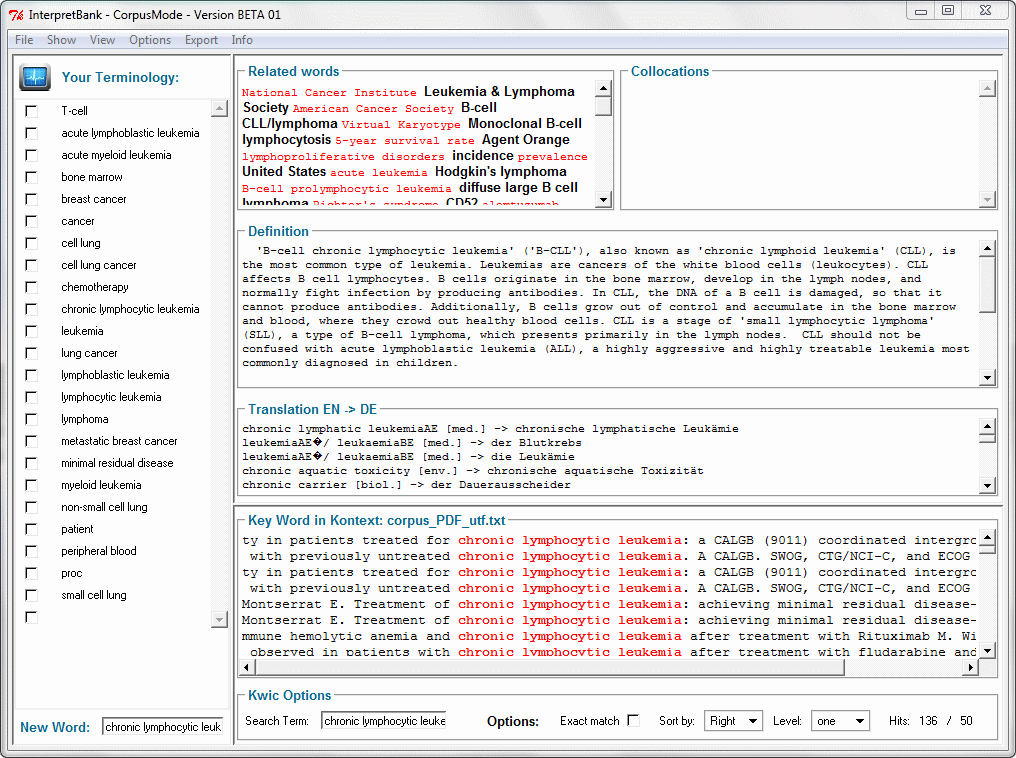
\includegraphics[width=\textwidth]{figures/FantinuoliF2.png}
\caption{Benutzeroberfläche von CorpusMode}
\label{fig:fantinuoli:2}
\end{figure} 

Der Workflow von CorpusMode beginnt mit der automatischen Sammlung relevanter Texte aus dem Internet zum Konferenzthema (\sectref{sec:fantinuoli:6.1.1}). Aus dem erstellten Korpus wird die Fachterminologie extrahiert (\sectref{sec:fantinuoli:6.1.2}), Definitionen und Übersetzungskandidaten zu jedem Terminus werden aus ausgewählten Quellen im Internet übernommen (\sectref{sec:fantinuoli:6.1.4}), verwandte Wörter und Kollokationen werden ermittelt (\sectref{sec:fantinuoli:6.1.5}). All diese Informationen werden schließlich auf einer integrierten Benutzeroberfläche (\figref{fig:fantinuoli:2}) angezeigt. Darüber hinaus bietet CorpusMode die Möglichkeit, Konkordanzen aus dem erstellten einsprachigen Korpus und aus frei verfügbaren Parallelkorpora zu analysieren (siehe \sectref{sec:fantinuoli:6.1.3}). Die Informationen, die mit CorpusMode erschlossen wurden, können anschließend mit dem eigenen terminologischen Werkzeug, TermMode, fixiert und für den späteren Gebrauch archiviert werden. 

\subsubsection{Automatische Erstellung einsprachiger Fachkorpora}\label{sec:fantinuoli:6.1.1}
\largerpage[-1]
CorpusMode sammelt automatisch fachspezifische, konferenzrelevante Texte -- die so genannten Paralleltexte -- aus dem Web und erstellt ein Fachkorpus. Die Idee, das Internet als Quelle für die Erstellung von Korpora zu verwenden, ist nicht neu und seit einigen Jahren Thema zahlreicher wissenschaftlicher Arbeiten \citep{Ghani2001,Baroni2004}: 

\begin{quote}
The Web is immense, free, and available by mouse click. It contains hundreds of billions of words of text and can be used for all manner of language research \citep[333]{Kilgarriff2003}.
\end{quote}

Das Internet kann als eine fast unendliche und leicht zugängliche Quelle linguistischer Daten betrachtet werden, die sehr gut geeignet ist, um \textit{disposable}\footnote{ Zur Bedeutung von \textit{Disposable Corpora}  \citet{Varantola2003}.} Korpora „on-the-run“ zu erstellen, vor allem Fachkorpora, die einmalig oder nur im Rahmen eines Projektes -- sprich einer Konferenz -- Verwendung finden\footnote{Zur Differenzierung von den unterschiedlichen Korporatypologien vgl. \citet{Hansen-Schirra2008} und \citet{Lemnitzer2010}.}.

Die grundlegende Funktionsweise ist einfach und basiert auf dem Ansatz von BootCaT \citep{Baroni2004}: Das Thema des Fachkorpus, welches gleichzeitig Konferenzthema ist, wird durch fünf oder sechs Termini festgelegt, die für die Konferenz relevant sind -- beispielsweise durch die Begriffe \textit{leukemia, bone marrow, chemotherapy, transplantation and acute lymphoblastic leukemia} bei einer Konferenz über \textit{Acute Leukemia}. Diese werden miteinander kombiniert und als Suchwörter bei einer Suchmaschine, in unserem Fall Bing\footnote{ ww.bing.com}, verwendet. Die von der Suchmaschine gefundenen PDF-Dokumente\footnote{Dabei werden die erweiterten Suchoptionen für die Suche nach bestimmten Formaten verwendet, in unserem Fall PDF-Dateien} werden heruntergeladen und als Text formatiert. Das Resultat dieses Prozesses ist ein einsprachiges Korpus, das Texte beinhaltet, die inhaltlich mit den Suchwörtern verwandt sind.\footnote{ Vgl. die Methode von BootCaT in \citet{Baroni2004}.} Als Quelle für diese Suchwörter können z.B. Konferenzprogramme dienen bzw. die Titel der einzelnen Vorträge oder Abstracts, die von den einzelnen Referenten gehalten werden und die meist schon einige Zeit vor der Konferenz zur Verfügung stehen. Um diesen Prozess noch weiter zu beschleunigen, können sich Dolmetscher dem Konferenzthema auch annähern, indem sie ein einziges Wort eingeben, das das Konferenzthema am allgemeinsten bezeichnet, z.B.\textit{ solar energy}, \textit{semiconductor} oder \textit{circuit design}. CorpusMode erstellt daraufhin nach der in \sectref{sec:fantinuoli:6.1.5} beschriebenen Methode automatisch eine Liste verwandter Wörter. Diese Termini werden dann als Suchwörter für die Suchmaschinenabfrage verwendet.

Vorteile dieser Methode, Korpora zu jedem beliebigen Thema automatisch zu erstellen, sind die Einfachheit und Schnelligkeit. In wenigen Minuten können Korpora mit hunderttausenden von Tokens erstellt werden. Nachteile sind dagegen die kaum vorhandenen Möglichkeiten der Kontrolle der gefundenen Texte. Unterschiedliche Tests haben jedoch ergeben, dass die Qualität der hergestellten Fachkorpora für die \textit{Corpus Driven Interpreter Preparation} sehr zufriedenstellend ist \citep{Fantinuoli2006}. Die Qualität hängt im Wesentlichen von der Auswahl der Suchwörter ab und kann somit vom Benutzter gesteuert werden \citep{Ueyama2006}. Die Möglichkeit, die gefundenen Texte auf Relevanz und Qualität zu überprüfen, ist dennoch gegeben.

Eine weitere Methode zur Erstellung eines Fachkorpus ist die kleine Software CorpusCreator, die ebenfalls Teil von InterpretBank ist. Mit dieser Software ist es möglich, Korpora aus PDF-Dateien auf der Grundlage einer Suchmaschinen-Suche zu erstellen.\footnote{Dabei kann eine beliebige Suchmaschine verwendet werden. Die hier angeführten Beispiele beruhen auf Suchvorgängen mit Google.} Der Nutzer benutzt z.B. die Suchmaschine Google und ihre leistungsfähige erweiterte Suche, um relevante Texte zu einem bestimmten Thema zu finden. Um ein englisches Korpus zum Thema Solarenergie zu erstellen, kann man zum Beispiel themenverwandte PDF-Dateien mit der folgenden Query finden: „solar cells filetype:pdf site:.com“\footnote{In Google begrenzt \textit{filetype} die Suche auf ein bestimmtes Dateiformat, \textit{site} auf eine bestimmte Internetdomäne.}. Um ein deutsches Korpus über die Unternehmenssprache der Firma Gehrlicher~AG zu erstellen, ist es möglich folgende Query zu benutzten: „filetype:pdf site:gehrlicher.com“. Die Internetseite mit den Suchergebnis wird als HTML-Datei auf der Festplatte des Nutzers gespeichert und von CorpusCreator verwendet, um alle gefundene PDF-Dateien automatisch herunterzuladen und in Text-Format zu konvertieren.
 
Die semi-automatisch erstellten Korpora werden für die Abfrage durch einen \textit{Concordancer} vorbereitet. Zuerst werden sie mit Metadaten angereichert. Das Markup enthält Informationen zu den Original-Dateien (Titel der Datei, URL, Timestamp, Kodierung, etc.). Dabei wird auf ein einfaches XML-Schema zurückgegriffen:

\ea
\begin{lstlisting}
<header>
  <filename></filename>
  <url></url>
  <encoding></encoding>
  <conversionTime></conversionTime>
</header>
\end{lstlisting}
\z

Das Korpus wird linguistisch mit morphosyntaktischen Merkmalen (Part-of-Speech Tagging) annotiert.
Hierfür wird ein POS-Tagger\footnote{Es wird der TreeTagger verwendet (\url{www.ims.uni-stuttgart.de/projekte/corplex/TreeTagger})} verwendet, d.h. eine Software, die in der Lage ist, jedes Token eines Textes einer bestimmten Wortklasse zuzuweisen. Auf weitere linguistische Annotationsebenen (syntaktische Annotation, semantische Annotation, Lemmatisierung, usw.) wird dagegen verzichtet, da diese in der Regel sehr zeitaufwendig ist und nur mit einem beträchtlichen manuellen Aufwand durchgeführt werden können. Die Flüchtigkeit der erstellten Korpora, die oft nur für einen einzigen Dolmetscheinsatz Verwendung finden, macht diese aufwendigen Annotationen unwirtschaftlich. Die Korpusabfrage erfolgt auf der Grundlage von Wortformen. Diese ist insbesondere für lexikografische Fragestellungen geeignet. Um die Abfrage zu unterspezifizieren, um zum Beispiel gleichzeitig nach verschiedenen Flexionsformen zu suchen, ist es möglich, nicht nur nach Wortformen zu suchen, sondern über reguläre Ausdrücke eine Mustersuche (wie z.B. Alteration, Gruppierung, Zeichenklasse, usw.) durchzuführen.\footnote{Für weitere Details zu den \textit{regular expressions} siehe \citet{Friedl2006}.}

\subsubsection{Automatische Extraktion von Fachterminologie}\label{sec:fantinuoli:6.1.2}

Die Fachterminologie einer Konferenz wird aus dem Fachkorpus (\sectref{sec:fantinuoli:6.1.1}) automatisch extrahiert. Die implementierte Extraktionsmethode basiert auf statistischen und linguistischen Ansätzen, die in einem Hybridverfahren kombiniert werden. Der statistische Ansatz beruht auf dem Vergleich der relativen Häufigkeit eines Tokens im Fachkorpus mit der relativen Häufigkeit desselben Tokens in einem Vergleichskorpus \citep{Rayson2000}. Anhand dreier unterschiedlicher statistischer Verfahren -- \textit{Weirdness Ratio}, \textit{Log Likelihood Ratio} und \textit{Log Odds Ratio}-- werden die typischen Tokens des Fachkorpus, also Einworttermini, identifiziert. Exemplarisch wird hier der Wert von der \textit{Weirdness Ratio} eines Tokens errechnet:

% \begin{equation*}
$$
\mathit{Weirdness}\mathit{Ratio}=(\mathit{Wspec}/\mathit{Tspec})/(\mathit{Wref}/\mathit{Tref})
$$
% \end{equation*}

\begin{quote}
Wspec = Häufigkeit des Tokens x im Fachkorpus
\end{quote}

\begin{quote}
Wref = Häufigkeit des Tokens x im Referenzkorpus 
\end{quote}

\begin{quote}
Tspec = Anzahl aller Token im Fachkorpus
\end{quote}

\begin{quote}
Tref = Anzahl aller Token im Referenzkorpus
\end{quote}


Aus dieser Formel ist ersichtlich, dass die \textit{Weirdness Ratio} einen höheren Wert haben wird, wenn die relative Häufigkeit des Tokens im Fachkorpus höher als im Referenzkorpus ist. Dies kann als Indikator dafür betrachtet werden, dass das Token typisch für das Fachkorpus ist.

Alle Tokens aus dem Fachkorpus werden schließlich in eine einzige Rangfolge gesetzt, indem man die Rangfolgen aus jedem einzelnen statistischen Verfahren miteinander kombiniert.\footnote{Vgl. das sogenannte „rank aggregation problem” \citep{DworkEtAl2001}.} Um die Qualität der extrahierten Einworttermini zu verbessern, wird außerdem die zuvor durchgeführte morphosyntaktische Analyse verwendet. Die Einworttermini, die statistisch identifiziert wurden, werden nun anhand von POS-Filtern selektiert. Somit können einzelne Wortklassen herausausgefiltert werden. In der Regel werden Substantive ausgewählt, da diese terminologisch am relevantesten sind. Die Möglichkeit, auch weitere Wortklassen zu extrahieren, z.B. Verben oder Adjektive, bleibt jedoch ebenso gewahrt. 

Mehrworttermini werden durch ein linguistisches Verfahren ermittelt. Aus dem mit POS-Tags angereicherten Korpus werden nach festgelegten Wortklassenmustern, wie z.B. für die englische Sprache „Noun + Noun“, „Adjective + Noun“ oder „Noun + Noun + Noun”, alle Mehrworttermini extrahiert, die den vorgegebenen Mustern entsprechen. Statistisch bereinigt wird diese Liste durch die Errechnung der relativen Häufigkeit dieser Kandidaten im Fachkorpus in Bezug auf deren Häufigkeit im Referenzkorpus. Das Ergebnis der Extraktion ist eine Liste von Einwort- und Mehrworttermkandidaten.

Die Bewertung der Qualität einer automatischen Terminologieextraktion hängt von ihrer Zielsetzung ab. Aus diesem Grund werden die Anzahl und der Typ der Termkandidaten, die in der Benutzeroberfläche angezeigt werden, nicht vorab festgelegt, sondern dem Nutzer überlassen. Damit die Software den unterschiedlichen terminologischen Bedürfnissen des Nutzers Rechnung tragen kann, ist es möglich, anhand eines sogenannten TerminologyEqualizers die Charakteristika der zu extrahierenden Termini zu bestimmen und somit die Zielsetzung der Extraktion anzupassen; beispielsweise können sich Benutzer nur hochspezifische Termini anzeigen lassen oder hochspezifische Termini plus allgemeinere Termini; nur Substantive oder Substantive plus Verben und Adjektive; usw. Durch diese Anpassbarkeit der Terminologieextraktion können Dolmetscher -- je nach Vorkenntnissen oder je nach den Sprachen, mit denen sie arbeiten müssen -- selbst entscheiden, welche Termini sie für eine optimale Vorbereitung des Einsatzes benötigen \citep{Fantinuoli2006}. Die Termextraktion wurde bis dato für die Sprachen English, Deutsch und Italienisch implementiert. Da die sprachlichen Ressourcen (z.B. die Parameterdateien des TreeTaggers) auch für andere Sprachen vorhanden sind, kann die Implementierung mit relativ geringem Aufwand auf andere Sprachen ausgeweitert werden.

\subsubsection{Einbindung von Parallelkorpora}\label{sec:fantinuoli:6.1.3}

Eine weitere Möglichkeit, dolmetschrelevante Informationen aus Textsammlungen zu gewinnen, besteht in der Untersuchung von Parallelkorpora, in denen Originaltexte ihren Übersetzungen in eine oder mehrere Zielsprachen zugeordnet sind. Diese werden generell benutzt, um Terminologie \citep{Pearson2003}, Kollokationen \citep{Teubert2003} und Valenzen \citep{culo_automatische_2011} automatisch oder manuell zu extrahieren. Beim professionellen Übersetzen und Dolmetschen können Parallelkorpora die Zahl der zur Verfügung stehenden sprachlichen Ressourcen ergänzen und vervollständigen.

\begin{quote}
A parallel corpus can be employed as a multilingual lexical resource, being more comprehensive and diverse than dictionaries \citep[1168]{Hansen-Schirra2008}.
\end{quote}

Eine der wichtigsten Eigenschaften von Parallelkorpora ist die Tatsache, dass die Originaltexte satzweise mit den Zieltexten aligniert sind, d.h. die Textteile (Sätze, Absätze, usw.) werden einander zugeordnet. Dies ermöglicht u.a. die parallele Darstellung vom Ausgangs- und Zieltext in einer für die manuelle Informationsgewinnung nützlichen Form (\figref{fig:fantinuoli:3}).

\begin{figure}
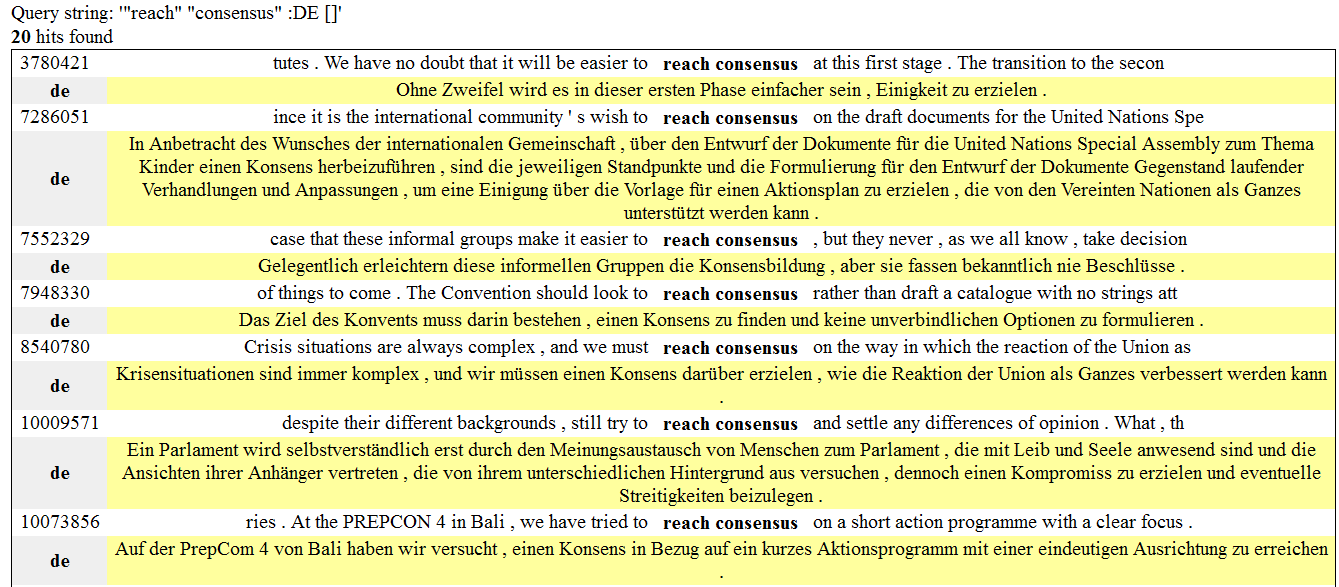
\includegraphics[width=\textwidth]{figures/FantinuoliF3.png}
\caption{Concordancer für Parallelkorpora am Beispiel von OpusCorpus}
\label{fig:fantinuoli:3}
\end{figure} 

Im Gegensatz zu den in \sectref{sec:fantinuoli:6.1.1} beschriebenen einsprachigen Fachkorpora, die ad-hoc für jedes neue Thema automatisch erstellt werden, integriert CorpusMode in die Software bereits aufbereitete Parallelkorpora. Der Grund liegt darin, dass es sehr aufwendig ist, frei verfügbare Texte im Web aufzubereiten und zu alignieren. Als Korpusquelle dient das Open Source Parallel Corpus\footnote{\url{http://opus.lingfil.uu.se/}}. Im OPUS-Korpus wurden frei zugänglich mehrsprachige Internetressourcen aligniert und in einem standardisierten XML-Format (TMX) als Downloaddatei zur Verfügung gestellt. Das Projekt stellt unterschiedliche Korpora bereit, wie z.B. \textit{ECB - European Central Bank corpus}, \textit{EMEA - European Medicines Agency documents}, \textit{EUROPARL -- European Parliament Proceedings}, \textit{OpenSubs -- the opensubtitles.org corpus}, etc. Die Korpora sind nicht linguistisch annotiert.\footnote{Für einen Überblick über linguistisch annotierte Parallelkorpora (Treebanken) siehe z.B. \citet{Hansen-Schirra2009}.} Die Suchmöglichkeiten bestehen daher aus reinen Zeichenketten. Zusammen mit den automatisch erstellten Korpora und den weiteren linguistischen Ressourcen (siehe \sectref{sec:fantinuoli:6.1.4} und \sectref{sec:fantinuoli:6.1.5}) können diese Parallelkorpora als zusätzliche Nachschlageressource verwendet werden, um sprachliche Informationen zu einem bestimmten Fachthema zu gewinnen. Vorteil der Einbindung von Parallelkorpora in CorpusMode ist die Möglichkeit, gezielt Übersetzungsvorschläge (z.B. Terminologie, Phraseologie, etc.) in dem gerade verwendeten Sprachpaar zu erhalten. Es sei an dieser Stelle angemerkt, dass CorpusMode in erster Linie für die Vorbereitung fachspezifischer Konferenzen gedacht ist. Die zur Zeit verfügbaren Parallelkorpora sind allerdings eher allgemeinsprachlicher Natur und können daher nicht alle möglichen Domänen abdecken. Obwohl die Zahl der frei verfügbaren Parallelkorpora in absehbarer Zeit steigen wird, wird sich ihr Nutzen weiterhin auf die Analyse allgemeinsprachlicher Phänomene beschränken. Dennoch kann dies für Dolmetscher von besonderer Bedeutung sein, vor allem im Hinblick auf die Suche nach Äquivalenzen in der Fremdsprache \citep{Fantinuoli2006}.

\subsubsection{Definitionen und Übersetzungsvorschläge für Fachtermini}\label{sec:fantinuoli:6.1.4}

Ein Korpus kann eine unerschöpfliche Quelle inhaltlicher und sprachlicher Informationen über ein Themengebiet sein. Es ist allerdings nicht immer die beste Ressource, wenn man z.B. nur nach der Definition eines Wortes sucht, wie Partington beobachtet:

\begin{quote}
Corpus examples give only contextual clues, from which it is not always easy to reconstruct the conceptual meaning of a word precisely, since speakers and writers tend to take it for granted that the hearer or reader will have a good idea of the conceptual meaning of most words used (\citeyear[64]{Partington2001}).
\end{quote}

Um das Informationsangebot aus der Korpusanalyse zu ergänzen, können auf der graphischen Benutzeroberfläche Zusatzinformationen zu einem Wort dargestellt werden. Das Web bietet nicht nur eine fast unendliche Anzahl an Texten, die zum Aufbau eines Korpus benutzt werden können; es stellt auch Informationen zur Verfügung, die für die Vorbereitung eines Dolmetscheinsatzes geeignet sind und schon heute zum Alltag eines jeden Dolmetschers gehören. Darunter fallen z.B. Enzyklopädien, Wörterbücher, terminologische Datenbanken, Expertenforen, etc. Das so genannte Web 2.0 erlebt seit einigen Jahren einen regelrechten Boom. Dabei handelt es sich um eine neue Generation des Webs, die durch eine Reihe interaktiver und kollaborativer Elemente charakterisiert ist. Durch den aktiven Beitrag der Webcommunity werden Webseiten zu \textit{Knowledge Repositories}, aus denen zahlreiche Informationen automatisch gewonnen werden können.\footnote{Für weitere Informationen zum Einsatz von Web 2.0 für NPL siehe z.B. \citep{Frank2008}.}

Zu den bekanntesten Web 2.0 Internetseiten gehört zweifelsohne Wikipedia,\footnote{\url{http://www.wikipedia.org}} deren Ziel der „Aufbau einer Universalenzyklopädie durch freiwillige und ehrenamtliche Autoren“ ist. Die große Anzahl der Artikel (die deutsche Version zählte Ende 2010 ca. 1.135.000 Artikel\footnote{Dieser Wert basiert auf der Angabe von Wikipedia, abrufbar unter \url{http://de.wikipedia.org/wiki/Wikipedia:\%C3\%9Cber\_Wikipedia} (abgerufen am 15.10.2010)}) stellt zusammen mit ihrer Interkonnektivität die Stärke dieses Dienstes dar. Wikipedia und ähnliche enzyklopädische Seiten bieten Dolmetschern die Möglichkeit, sich rasch in ein Thema einzuarbeiten und damit „a mental representation of incoming text on the basis of previous knowledge“ \citep[777]{Kalina2005} zu bilden. Der Mangel an Maßnahmen zur Qualitätssicherung der Beiträge wird allerdings von mehreren Wissenschaftlern bemängelt, so dass Nutzer dieser Ressource oft kritisch gegenüber stehen. So prüfte \citet{Lorenz2009} in der deutschsprachigen Wikipedia z.B. alle 285 Einträge zum Thema Zahnmedizin auf ihre medizinisch-wissenschaftliche Qualität. 16\% der Artikel enthielten demnach inhaltliche Fehler und waren nicht geeignet, aktuelles zahnmedizinisches Fachwissen zu verbreiten. Der Rest wurde als qualitativ mit einem Lehrbuch vergleichbar eingestuft (28\%) oder vermittelte richtiges Wissen, ohne jedoch von der Qualität der Darstellung her einem Lehrbuch ebenbürtig zu sein (56\%). Diese Untersuchung zeigt, dass trotz der unwiderlegbaren Problematik eines Teils der Artikel 84\% der Informationen brauchbar sind. Eine offene Plattform wie Wikipedia kann demnach als geeignete Informationsquelle betrachtet werden. Der Gebrauch solcher Informationen seitens der Dolmetscher dient im Grunde genommen jedoch ohnehin nur der Aneignung eines Grundwissens, die es ihnen ermöglicht, konferenzspezifische Texte zu verstehen. Die verschiedenen Perspektiven eines Anwenders, der Wikipedia als Einstieg in ein Thema verwendet, und eines anderen Nutzers, der nicht nur einen Überblick über die Begrifflichkeit bekommen möchte, sondern die konkreten Informationen in seine Arbeit einbeziehen bzw. umsetzen möchte (z.B. ein Arzt), relativiert die Gewichtung qualitativ nicht hochwertiger Artikel.

Über diese offenen, kollaborativen Angebote hinaus bieten viele Internetseiten außerdem Zugang zu traditionellen Wörterbüchern und lexikalischen Datenbanken, die im Umfang kleiner als Web 2.0 Anwendungen sind, aber einen hohen Qualitätsanspruch haben. Als Beispiel kann an dieser Stelle das englische WordNet\footnote{\url{http://wordnet.princeton.edu/}} der Universität Princeton erwähnt werden.

Wie die oben aufgeführten enzyklopädischen und lexikalischen Informationsquellen ist auch die Zahl der Online-Ressourcen, die Übersetzungen von Termini anbieten, sehr groß. Man denke z.B. an die Internetseiten BEOLINGUS der TU Chemnitz\footnote{\url{http://dict.tu-chemnitz.de}}, leo.de\footnote{\url{http://www.leo.de}}, dict.cc\footnote{\url{http://www.dict.cc}} oder IATE\footnote{\url{http://iate.europa.eu}}, die mehrsprachige Terminologie-Datenbank der Europäischen Union. Auch hier gelten dieselben Einschränkungen zur Qualität, die man bei enzyklopädischen Ressourcen wie Wikipedia feststellen muss. Dennoch bieten sie dem professionellen Sprachmittler Übersetzungsvorschläge, die als Basis für eine weiterführende terminologische Recherche dienen können. 

All diese Ressourcen werden heutzutage von den meisten Dolmetschern schon eingesetzt. Da sie in vielen Fällen unter einer Creative-Commons-Lizenz sowie einer GNU-Lizenz für freie Dokumentation freigegeben sind (wie z.B. Wikipedia), ist es möglich, diese Informationen in eine einzige Benutzeroberfläche zu bündeln und mit vorhandenen zusätzlichen Ressourcen, etwa die extrahierte Fachterminologie, zu kombinieren. Ausgehend von einem konferenzrelevanten Terminus kann der Nutzer somit direkt auf Definitionen und Übersetzungsvorschläge zugreifen, die ihn bei der inhaltlichen und sprachlichen Vorbereitung unterstützen können.

\subsubsection{Verwandte Termini und Kollokationen}\label{sec:fantinuoli:6.1.5}

Durch die Visualisierung eines semantischen Netzes, das ausgehend von einem \textit{Node} verwandte Worte abbildet, können Brainstorming-Aktivitäten gefördert werden. Brainstorming ist eine Strategie, die verwendet wird, um bereits gespeicherte Informationen im Gehirn zu aktivieren oder um Wissen durch neue Informationen zu erweitern. Dies geschieht, indem man assoziativ an Begriffe und Benennungen denkt, die mit einem Ausgangsthema semantisch und inhaltlich verwandt sind \citep{Osborn1957}. Dieser Ansatz des assoziativen Lernens kann in einem den Dolmetschern nicht vertrauten Thema durch die Bereitstellung thematisch verwandter Begriffe und Kollokationen erfolgen.\footnote{Zur Rolle des Brainstorming bei der interlingualen Übersetzung, dem Zugang zu „common concepts” und der „activation of concepts“, \citet{Blot2003}.} \citeauthor{Zock2010} argumentiert, dass „Information access depends crucially on the organization of the data (words) and the access keys (meaning/form), two factors largely overlooked“ (\citeyear[201]{Zock2010}). Um dieses Problem zu überwinden, bietet sich die Anwendung von Wordclouds an, die den Zugang zu neuen Termini erleichtern und dynamischer gestalten können. 

\begin{figure}
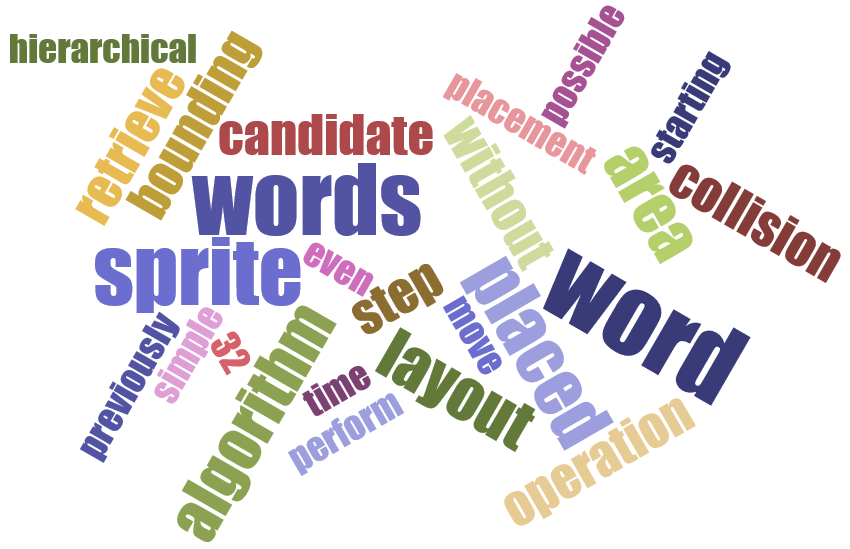
\includegraphics[width=\textwidth]{figures/Fantinuoli-wordcloud_neu.png}
\caption{Wordcloud}
\label{fig:fantinuoli:4}
\end{figure} 

Ein semantisches Netz, das einen extrahierten Fachterminus als Ausgangspunkt hat, lässt sich beispielsweise bilden, indem man die Vernetzung der Einträge in Wikipedia nutzt, um semantisch verwandte Wörter zu extrahieren. Durch das Parsing des HTML-Codes eines bestimmten Eintrages ist es möglich, alle als Link markierten Benennungen zu identifizieren und als Grundlage für die Darstellung des semantisches Netzes zu verwenden. Da diese Wörter von der Wikipedia-Community als Links zu weiterführenden Artikeln markiert wurden, sind sie de facto Termini, die mit dem Node -- d.h. dem ursprünglichen Artikel -- verwandt sind. Diese Brainstorming-Aktivität kann auch durch die Bereitstellung von Kollokationen ergänzt werden, denn: 

\begin{quote}
Ein standardmäßiges Nachschlagen in der aufkommenden Gattung von Kollokationswörterbüchern mit einem Vorschlag der üblichsten Kollokatoren wird sicherlich die Antizipation beim Simultandolmetschen erleichtern, ebenso wie die Differenzierungsfähigkeit \citep[58]{Stoll2009}.
\end{quote}

Die Art der Darstellung dieser Termini ist in \figref{fig:fantinuoli:4} zu sehen. Die einzelnen Termini fungieren demnach als „Access Keys“ bzw. als „an index based on the notion of association“  \citep[201]{Zock2010}, um das Thema der Konferenz weiter zu vertiefen oder um bereits vorhandene Kenntnisse vor einem Einsatz wieder zu aktivieren.

\subsection{Terminologie verwalten: TermMode}\label{sec:fantinuoli:6.2}

Während terminologische Daten und fachliche Informationen lange Zeit auf Papier verfasst und verbreitet wurden, bieten computerlinguistische Anwendungen und das Internet neue Möglichkeiten der Datenverarbeitung und -darstellung. Die Verfügbarkeit großer Datenmengen, die dynamische Datendarstellung und die unterschiedlichsten Möglichkeiten des Datenzugriffs mittels ausgereifter Suchverfahren sind nur einige der wichtigen Vorteile der elektronischen Datenverarbeitung.

Die starre und meist normative Struktur gedruckter lexikografischer Werke wie z.B. Wörterbücher und Lexika überlassen den dynamischen und linguistisch deskriptiven Ansätzen der computerunterstützten Wissens- und Terminologieverwaltung das Feld. Die Vernetzung kontrollierter Datenbestände (Glossaren) mit automatisch gesammelten Fachtexten (6.1.1) sowie die Einbindung von Datensammlungen in speziell für die Bedürfnisse der Nutzer programmierten Anwendungen (\sectref{sec:fantinuoli:6.1.4} und \sectref{sec:fantinuoli:6.1.5}) können die Möglichkeiten der \textit{Knowledge Experience} -- der Aneignung von Wissen und Terminologie -- erweitern und ergänzen \citep{Fantinuoli2009}. 

\largerpage
In diesem Zusammenhang kommt das Terminologieverwaltungsmodul von InterpretBank namens TermMode zum Einsatz. Mehrsprachige Glossare werden in einer SQLite-Datenbank gespeichert. Neben der Möglichkeit, eine Benennung in mehreren Sprachen zu registrieren, ermöglicht die Software es auch, weitere Informationen zu einem Begriff zu speichern wie z.B. Kollokationen, Definitionen, etc. Alle Glossare werden in einer einzigen Datenbank verwaltet und mittels zweier Klassifikatoren gegliedert, nämlich \textit{Glossar} und \textit{Konferenz}. Speziell auf die Dolmetscher zugeschnittene Felder sind in der Benutzeroberfläche integriert; so kann das Feld \textit{ConfInfo} z.B. dazu genutzt werden, simultanrelevante Informationen zu speichern, um diese in der Kabine mit ConferenceMode zusammen mit den Benennungen abzurufen.

Die ergonomische Darstellungsstruktur ist modularisiert, d.h. an die jeweiligen Bedürfnisse des Nutzers anpassbar. Somit kann die Bedienungsoberfläche geändert werden: Von einer vereinfachten Eintragsstruktur, in der nur die jeweiligen Benennungen eingetragen werden können (\figref{fig:fantinuoli:5}), in eine komplexere Struktur, die es erlaubt, Zusatzinformationen zu einem Begriff einzugeben (\figref{fig:fantinuoli:6}). Diese Expansionsfähigkeit ist stufenweise einstellbar. 

\begin{figure}
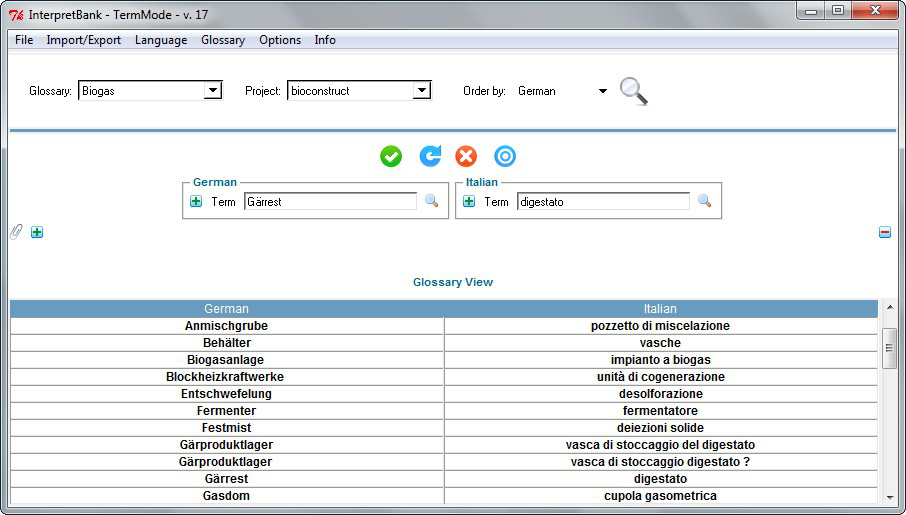
\includegraphics[width=\textwidth]{figures/FantinuoliF5.png}
\caption{TermMode, einfache Eintragungsstruktur}
\label{fig:fantinuoli:5}
\end{figure} 

\begin{figure}
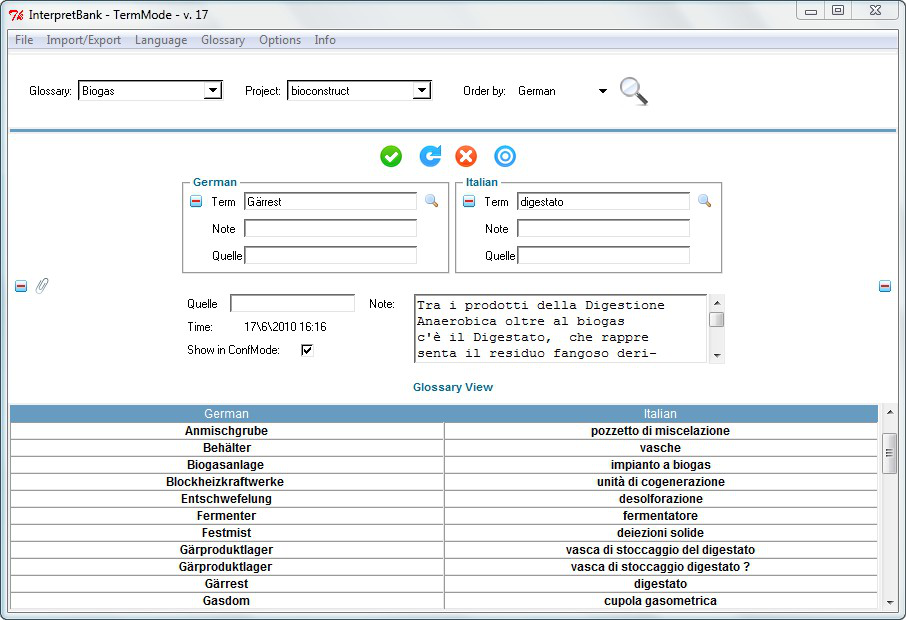
\includegraphics[width=\textwidth]{figures/FantinuoliF6.png}
\caption{TermMode, erweiterte Eintragungsstruktur}
\label{fig:fantinuoli:6}
\end{figure} 

\largerpage
Die Visualisierung der Glossare erfolgt in tabellarischer Form und entspricht somit der klassischen Darstellungsform, wie sie von Dolmetschern und Übersetzern typischerweise für ihre Glossare verwendet wird. Darüber hinaus ist das Modul mit CorpusMode dynamisch verbunden: Die Termkandidaten, die von einem Fachkorpus extrahiert wurden, können z.B. automatisch in TermMode importiert werden. Außerdem kann der Nutzer, ausgehend von einem Eintrag im Glossar, zusätzliche Informationen wie Konkordanzen, Definitionen, verwandte Wörter, usw. direkt in TermMode abrufen. Anders als bei traditionellen Terminologieverwaltungssystemen wird so der Zugang zur Terminologie mit TermMode dynamischer: Die Informationen, die dem Nutzer zur Verfügung stehen, sind nicht mehr nur auf diejenigen Informationen beschränkt, die man in eine klassische Eintragungsstruktur manuell eingepflegt hat, sondern werden durch die projektbezogenen Ressourcen erweitert, die durch CorpusMode bereit gestellt wurden. 

\subsection{Terminologie abrufen: ConferenceMode}\label{sec:fantinuoli:6.3}

ConferenceMode ermöglicht Konferenzdolmetschern in der Kabine den schnellen und bedarfsorientierten Zugriff auf bestehende mehrsprachige Terminologiedaten, d.h. auch während der Verdolmetschung. Aufgrund der Besonderheiten des Dolmetschprozesses in einer Simultansituation muss die Anwendung für den Einsatz in der Kabine vor allem Wert auf die folgenden Grundbeschaffenheiten legen \citep{SDI2007}:

\begin{itemize}
\item  
schnelle und flexible Suchfunktion 
\item  
Übersichtlichkeit 
\item  
komfortable und schnelle Eingabe neuer Termini 
\item  
intuitive Bedienbarkeit 
\item  
Kompatibilität mit anderen Programmen 
\end{itemize}

\newpage 
ConferenceMode verwendet eine interne Datenbank, das so genannte \textit{Activ Glossary}. Diese Datei enthält alle Wortpaare und Zusatzinformationen, die im Vorfeld für einen Einsatz geladen wurden und bleibt unverändert, bis ConferenceMode für den nächsten Einsatz mit einem anderen Glossar geladen wird. Diese Lösung ermöglicht es Dolmetschern, das \textit{activ Glossary} individuell zusammenzustellen, indem sie ein oder mehrere Glossare aus TermMode oder aus anderen Programmen (MS~Word, MS~Excel, SDL~Multiterm, etc.) nacheinander laden. Dank dieser hohen Flexibilität können Dolmetscher sogar am Einsatzort schnell und unproblematisch Glossare von Kunden oder Kollegen einlesen und zum aktiven Glossar hinzufügen, ohne komplizierte Importfunktionen durchführen zu müssen. 

Die Idee, Fachglossare auch während der Verdolmetschung nachzuschlagen, ist nicht neu \citep{Stoll2002} und wird einerseits durch die Vorverlagerung der kognitiven Prozesse in die Vorbereitungsphase ermöglicht -- was die Dolmetscher während der Verdolmetschung entlastet (siehe \sectref{sec:fantinuoli:2}) -- anderseits durch die Tatsache, dass Dolmetscher die Einträge eines Glossars (meist) selbst in das Terminologieverwaltungssystem eingetragen haben, wobei „die gefundenen Äquivalenzen nur noch reaktiviert“ werden \citep[18]{Drechsel2005}. ConferenceMode fungiert somit eher als eine Gedächtnisstütze denn als Gedächtnisersatz. 

\begin{figure}
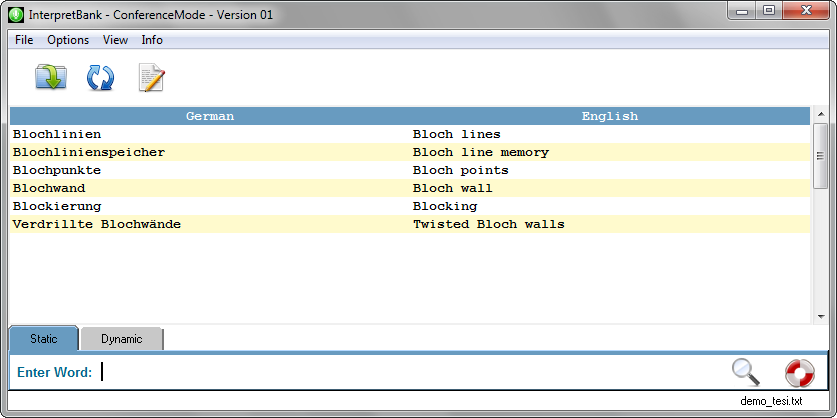
\includegraphics[width=\textwidth]{figures/FantinuoliF7.png}
\caption{ConferenceMode, kabinenfreundliches Nachschlagen während der Konferenz}
\label{fig:fantinuoli:7}
\end{figure} 

Um den Dolmetschprozess so wenig wie möglich zu beeinträchtigen und die Dolmetscher bei der Suche nach passenden Fachbegriffen auch während der Verdolmetschung optimal zu unterstützen, ist es notwendig, den kognitiven Aufwand für die Benutzung des Tools niedrig zu halten. Dafür muss einerseits der erforderliche Input seitens des Nutzers so klein wie möglich sein, andererseits muss der Output, d.h. die Ergebnisse einer Suchoperation, so übersichtlich wie möglich dargestellt und in der Anzahl auf ein Minimum reduziert werden. Idealerweise sollten die Dolmetscher also mit wenig Aufwand möglichst wenige, aber gleichzeitig relevante Treffer angezeigt bekommen, damit sie von der Suchoperation nicht abgelenkt werden. In ConferenceMode wird der gesuchte Begriff mittels Tastatur eingegeben, während die Suche mit der Entertaste oder mit einem Suchalgorithmus (ohne Entertaste) begonnen wird. Der Suchalgorithmus ermöglicht das Anzeigen der relevanten Treffer schon während der Eingabe. Bei jedem neuen Buchstaben, der eingetippt wird, werden die Ergebnisse entsprechend reduziert. Sobald die voreingestellte Anzahl von Treffern angezeigt wird (standardmäßig fünf Treffer), wird die Suche beendet und die Eingabemaske für eine weitere Suche freigegeben. 

Die Reduzierung der angezeigten Treffer erfolgt u.a. durch den Einsatz von Stopwords. Wenn man z.B. nach dem Wort „Dermatologie“ sucht und die Buchstabenkette „d“, „de“ oder „der“ eingibt, wird der Eintrag „Entzündung der Bauchspeicheldrüse“ nicht angezeigt, weil der Artikel „der“ auf die Stopwordliste gesetzt wurde. Man geht dabei davon aus, dass Nutzer nur nach bedeutungstragenden Wörtern suchen, so dass sie bei dem Terminus „Entzündung der Bauchspeicheldrüse“ entweder nach dem Wort „Entzündung“ oder „Bauchspeicheldrüse“ suchen würden. Darüber hinaus korrigiert der Suchalgorithmus mögliche Tippfehler bei der Eingabe der Zeichenkette (Suchwort) und in den Termini, die im Glossar gespeichert sind. Dafür wurde die Fuzzy-Match-Korrektur nach dem Prinzip der Levenshtein-Distanz implementiert. Aufgrund der Spontaneität der Suche und der Besonderheit der Situation, in der diese stattfindet, ermöglicht die Behebung dieser möglichen Fehlerquelle eine weitere Entlastung für die Dolmetscher, die, anders als Übersetzer, eine fehlgeschlagene Suche aus Zeitgründen nicht mehr wiederholen können. Dank dieser interaktiven Suchmethode werden Dolmetscher bei der Suche erheblich entlastet, da sie einen kleineren kognitiven Aufwand investieren müssen (Reduzierung der zu betätigenden Tasten, Darstellung nur weniger Treffer, etc.).

Während des Einsatzes haben Dolmetscher oft die Möglichkeit, ihr terminologisches Wissen durch neu gewonnene Informationen zu ergänzen. Damit die Eingabe neuer Termini während des Einsatzes schnell und komfortabel erfolgen kann, ist es möglich, auf eine dedizierte Eintragungsmaske zurückzugreifen, um neue Termini oder Anmerkungen zu schon vorhandenen Termini zu ergänzen. Die neuen Termini werden direkt zu dem aktiven Glossar hinzugefügt, so dass diese in der Kabine gleich abrufbar sind. Zudem werden sie automatisch in TermMode aufgenommen, damit sie ordnungsgemäß gespeichert werden und nicht verlorenen gehen.

\begin{figure}
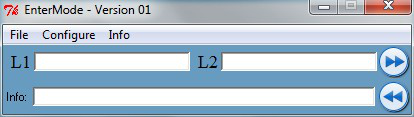
\includegraphics[width=\textwidth]{figures/FantinuoliF8.png}
\caption{TermMode, schnelles Eintragen neuer Termini während der Konferenz}
\label{fig:fantinuoli:8}
\end{figure} 

Wie in \sectref{sec:fantinuoli:6.2} erwähnt, kann die reine zweispaltige Darstellung in ConferenceMode mit den zweisprachigen Benennungen um eine dritte Spalte mit allgemeinen Informationen erweitert werden, die von den Dolmetschern als konferenzrelevant erachtet werden. In dieser Spalte können beispielsweise Informationen zur Verwendung eines Begriffs hinzugefügt werden.

Zu den weiteren Funktionen von ConferenceMode gehören die Anpassung der Suchfunktion beim bidirektionalen Dolmetschen, die Suche -- durch die \textit{EmergencySearch} -- in der gesamten TermMode-Datenbank sowie die Möglichkeit, besondere Zeichen wie z.B. diakritische Zeichen bei der Suche zu ignorieren.

\section{Schlusswort}\label{sec:fantinuoli:7}

Während Softwareanwendungen seit Jahren zu einem festen Bestandteil des Übersetzerberufs geworden sind, bleibt die Praxis des Dolmetschens von den neuesten Entwicklungen und Erkenntnissen im Bereich Computer- und Korpuslinguistik weiterhin unberührt. Da die möglichen Vorteile des computergestützten Dolmetschens vor, während und nach der Verdolmetschung auf der Hand liegen, versucht das Projekt InterpretBank, eine erste Brücke zwischen den terminologie- und korpusorientierten Ansätzen in der Dolmetschwissenschaft und dem „state-of-the-art“ in der Computerlinguistik zu schlagen, damit praktizierenden und angehenden Dolmetschern die Möglichkeit eingeräumt wird, auf ein Tool zurückgreifen zu können, das die Qualität ihrer Dienstleistung steigert. 

\end{otherlanguage}
{\sloppy 
\printbibliography[heading=subbibliography,notkeyword=this]
}
\end{document}

